\documentclass[11pt, a4paper]{article}

\usepackage{cite}

\usepackage{booktabs}
\usepackage{siunitx}
\DeclareSIUnit{\calorie}{cal}

\usepackage{pgfplots}
\usepackage{pgfplotstable}
\pgfplotsset{compat=newest}

\usepackage{physics}

\usepackage{amsmath}
\usepackage{tikz}
\usetikzlibrary{positioning, calc}

\pgfmathsetmacro{\s}{0.5}
\pgfmathsetmacro{\r}{0.5cm}

\usepackage[caption=false]{subfig}


\title{Predicting the binding free energy of DNA intercalators}
\author{Kristof Farkas-Pall}

\begin{document}

% \maketitle

\section*{Abstract}

Planar aromatic molecules can interact with DNA chains by intercalating between consecutive basepairs. Once intercalated they can cause mutations during gene expression resulting in cancerous cells. This same mechanism renders some of these molecules good anti-cancer treatment if targeted correctly. The efficacy of intercalators is therefore of importance to the pharmaceutical industry. However due to forcefield inadequacy and the slow convergence of computational simulations, the application of well established binding free energy calculation methods to DNA-intercalator system to predict efficacy has been low in number compared to protein-ligand studies. Here we apply the three main methods to predicting efficacy via computational methods to DNA intercalator systems comparing results to experiment. We found that docking methods are capable to distinguish between intercalators that have different scaffold structures, MMPBSA type simulations can correctly rank a congeneric series of intercalators, and formally exact methods predict the binding affinity of intercalators with root mean squared error of 0.41 kcal/mol. The correct preparation of the models was also important, and to this end we developed computational tools to automate the correct setup stages. With an automated setup and deployment tool and running our protocols we think will start to probe a wide range of intercalators to investigate their interaction and efficacy with DNA.

\section{Introduction}


\chapter{Methods}

\section{Experimental measurements of intercalation}

(~for example through displacement assays (move to experimental section, experimental difficulties, why is it hard to measure DNA intercalator biding affinity)~). ~Here we looked at a congeneric series intercalators based on a common quinoxaline scaffold with experimental measurements \cite{}.(Move to methods)~

\begin{figure}[h]
	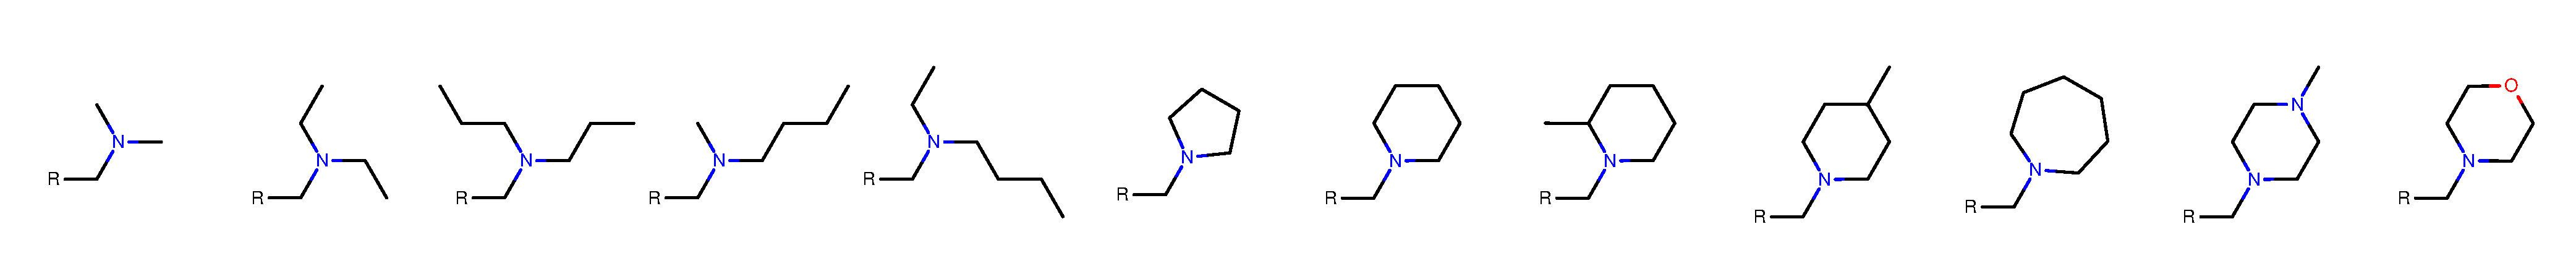
\includegraphics[width=\textwidth]{intercalators.pdf}
	\caption{A congeneric series of DNA intercalators. All molecules share a common quinoxaline scaffold. ~The experimental study was conducted by \cite{} producing binding affinity values that we could compare our calculations to. (Mention it in the experimental section)~ }
	\label{fig:intercalators}
\end{figure}


\section{Docking and scoring}

For certain application, like that of high throughput screening in the pharmaceutical industry, it is important to assess the binding strenght of a large number of drugs or molecules bound to large biological macromolecules like proteins or DNA in a very fast manner. This is done via easily evalutable scoring function, some notable examples including: AutoDock, X-Score, DrugScore, ChemScore, GOLD, FlexX, LigScore and LUDI. Generally speaking, they take into account a single structure and little or no protein movement is taking into account during evaluation. One of the simplest scoring function  consists of the empirical surface-area based method that shows that ligand binding reduces the surface are in the receptor that is accessible to the surrounding solvent. The function makes the assumption that the polar and non-polar area on the surface of the molecule has a linear relation to the free energy. Due to the crude simplifications in these models, they have weak predictive power and are rarely used for accurate free energy estimation. Here, a scoring methods is used for two reasons: (i) to find an initial structure for the intercalator-DNA complex, and (ii) to compare the scores and hence the ranking of this methods with other, more accurate models. Docking and scoring has its place in the drug discovery pipeline. In high throughput scenarios, where speed is an important factor due to the large number of molecules that need to be tested, scoring functions are often used to filter out candidates that have low probability of being good binders.

\subsection{Starting structures for docking}



\subsection{MMPBSA}

Molecular Mechanics Poisson-Boltzmann Surface Area (MMPBSA) is one of the theoretically approximate methods to calculate the free energy of system \cite{gilson2007calculation, steinbrecher2010towards}. It is the most accurate of the approximate methods, and it has previously been applied successfully to the free energy calculation of various biological systems including protein-ligand and DNA intercalator complexes.

This method is a good choice for comparing and ranking a set of molecule by their binding affinities for two main reasons: MMPBSA is able to handle a wide variety of systems and can the results can be theoretically calculated from a a single trajectory, unlike theoretically exact alchemical methods like FEP or TI. 

MMPBSA has become the a popular method to calculate binding affinities because of a balance between the details included in the physical model and the speed of the calculations themselves \cite{kollman2000calculating, sitkoff1994accurate}. As one of the main methods used in this thesis to calculate DNA-intercalator interactions, it will be discussed in more detail.

Applying the MMPBSA method to a system involves calculating the absolute free energy of binding by calculating three separate components: the free energies of the DNA-intercalator complex, the DNA and the intercalator molecules alone. The change is free energy upon intercalation then is

\begin{equation}
  \Delta G = \langle G_{complex} \rangle - \langle G_{DNA} \rangle - \langle G_{intercalator} \rangle
\end{equation}
\label{eq:mmpbsa}

where $\langle \dots \rangle$ represent the average value of a post-processing calculation performed on every frame of the simulation trajectory. Simulations are performed in explicit solvent and with counter-ions to balance the charge in the periodic simulation box.
To aid faster convergence of the free energy values the MMPBSA methods employs two strategies: first, all solvent molecules and counter-ions are replaced from the trajectory post simulation but pre-analysis by a continuum solvent approximation, and a thermodynamic cycle is used.

\subsubsection{The thermodynamic cycle}

\begin{figure}
  \centering
  \begin{tikzpicture}
  [ 
  waterbox/.style={rectangle,draw=blue!50,fill=blue!10,thick, inner sep=0pt,minimum size=5*\r},
  dna/.style={ultra thick, line cap=round},
  intercalator/.style={dna, dna, line width=3pt, blue},
  pre/.style={<-,shorten <=1pt,shorten >=1pt,semithick}, 
  post/.style={->,shorten <=1pt,shorten >=1pt,semithick}
  ]
  
  \node[waterbox] (a)               {};
  \node[waterbox] (b)  [right=of a] {}
    edge [pre] node[auto, swap] {$\Delta G_\text{b}^{aq}$} (a);
  \node[waterbox, fill=white] (a') [below=of a] {}
    edge [post] node[auto] {$\Delta G_\text{intercalator}^{sol}$} (a);
  \node[waterbox, fill=white] (b') [below=of b] {}
    edge [pre] node[auto] {$\Delta G_\text{b}^{vac}$} (a')
    edge [post] node[auto] {$\Delta G_\text{complex}^{sol}$} (b);
  \node[waterbox] (c)  [left=of a] {};
  \node[waterbox, fill=white] (c') [left=of a'] {}
    edge [post] node[auto] {$\Delta G_\text{dna}^{sol}$} (c);
    
  \node at ($(c.center)!0.5!(a.center)$) {+};
  \node at ($(c'.center)!0.5!(a'.center)$) {+};
  
  % \node[text width=10cm, align=center] [above=of a] {Thermodynamic cycle used to indirectly calculate the absolute free energy of intercalation};
  
  
  \foreach \x in {b.center, b'.center, c.center, c'.center} {
    \draw[dna]
      (\x) [rounded corners=\r] -- ++(-\s, 0) -- ++(0, 2*\s) 
      (\x) [rounded corners=\r] -- ++( \s, 0) -- ++(0, 2*\s)
      (\x) [rounded corners=\r] -- ++(-\s, 0) -- ++(0,-2*\s)
      (\x) [rounded corners=\r] -- ++( \s, 0) -- ++(0,-2*\s)
      
      (\x) ++(-0.866*\s,  0.5*\s) -- ++(1.73205*\s, 0)
      (\x) ++(   -\s,      \s) -- ++(   2*\s, 0)
      (\x) ++(   -\s,  1.5*\s) -- ++(   2*\s, 0)
      
      (\x) ++(-0.866*\s,  -0.5*\s) -- ++(1.73205*\s, 0)
      (\x) ++(      -\s,      -\s) -- ++(      2*\s, 0)
      (\x) ++(      -\s,  -1.5*\s) -- ++(      2*\s, 0);
  }
  
  \draw[intercalator] (a.center)  ++(-0.8*\s, 1.25*\s) -- ++(1.6*\s, 0);
  \draw[intercalator] (b.center)  ++(-0.8*\s, 1.25*\s) -- ++(1.6*\s, 0);
  \draw[intercalator] (a'.center) ++(-0.8*\s, 1.25*\s) -- ++(1.6*\s, 0);
  \draw[intercalator] (b'.center) ++(-0.8*\s, 1.25*\s) -- ++(1.6*\s, 0);

\end{tikzpicture}
  \caption{A solvation thermodynamic cycle is used to indirectly calculate the absolute binding free energy, $\Delta G_{b}^{aq}$, of an intercalator to the DNA in solvent. The rest of the free energy changes are calculated or estimated to then compute free energy of intercalation.}
  \label{fig:mmpbsacycle}
\end{figure}


\subsubsection{Single and Component trajectories}

The different contributions in equation \ref{eq:mmpbsa} can be extracted from a single trajectory of the complex, or from separate trajectories of the DNA, intercalator and complex. If a single trajectory is used, then the during the calculation of the different component, the rest of the system is removed and the analysis is done on part of the trajectory. This approach is effective in most scenarios and saves the additional cost of running multiple simulations for the separate components\cite{foloppe2006towards, wang2001use}. The other advantage of the single trajectory approach is that part of the complex that do not affect the intercalation cancel out exactly, as the coordinates are taken from the same trajectory, hence they are exactly the same. If separate trajectories are run for each component, than this error cancellation does not occur, as the component are free to explore different conformations. On the other hand, a single trajectory will not be able to capture dynamical changes to either the intercalator or, more importantly to the DNA, upon intercalation, and will consequently ignore certain contributions to the binding free energy. In the rest of the thesis, the three possible trajectory approaches are termed 1, 2 and 3 trajectory, corresponding to MMPBSA calculations where all three components are from the same simulation (1 trajectory), the intercalator is from a separate simulation (2 trajectory), or all three components, including the DNA are from three separate simulations (3 trajectory). 


\section{TIES}

The complexes of target DNA and hybrid intercalators were solvated in an orthorhombic water box with buffer width of 11 angstrom. The system was neutralized electrostatically with counterions. The BSC1\cite{ivani2016parmbsc1} force field was employed in all our simulations for DNA parameters. Intercalator parameters were produced using the general AMBER force field 2 (GAFF2) \cite{wang2004development}. The AM1BCC \cite{jakalian2002fast} %
semi-empirical methods was used to produce the partial charges on the intercalator atoms (AmberTools 18 \cite{ambertools18}) after geometry optimization with the OpenEye OEGauss toolkit. The simulation engine NAMD 2.12 was used for producing all the trajectories of the complex systems with periodic boundary conditions. The system was brought to and maintained at a temperature of 300 K and 1 atmosphere using the NAMD implementation of the Langevin thermostat (with a damping coefficient of $5 ps^{-1}$) and a Berendsen barostat (compressibility of $4.57 \times 10^{-5} bar^{-1}$ and a relaxation time of $100 fs$). The time step was set to $2 fs$. The van der walls terms perturbed linearly with respect to $\lambda$. To avoid end point catastrophes were atoms near the end point appear suddenly too close to each other a soft core potential was used for the van der Walls interactions. The electrostatic interactions of the disappearing atoms are linearly decoupled until $\lambda = 0.55$ then completely turned off afterwards, and those atoms that are appearing are electrostatically turned on from $\lambda = 0.45$ linearly increasing until the end.

All calculations were done with 13 $\lambda$ windows. At each value of $\lambda$ 5 replica simulations were run to assess the error. For each replica, the standard protocol for minimisation and equilibration was performed, that is 4 ns of simulation time. Production runs for each replica were 16 ns long. While the coordinates were recorded every 10 ps, $\partial V / \partial \lambda$ values were recorded every 2 ps. The choice of 16 ns for the simulation length and 5 for the ensemble size is based on the uncertainty quantification and error analysis discussed in the previous work. The protocol described here can be adjusted to the specific system at hand, but this was enough to converge results for all of the systems in this study. The size of the ensemble can be adjusted even at specific windows to account for additionally uncertainty that may arise. The TIES workflow can be executed in an embarrassingly parallel fashion, and given sufficient resources the simulations can finish in 15 hours. In general the turnaround time depends on the system size, number of cores used per simulation instance with GPUs offering additional speedup.



\chapter{Results and discussion}

This chapter describes and discusses the results. The results for each of the computational approaches to estimate either the binding free energy directly or range the intercalators is presented first, followed by a discussion of their relative merits.


\section{Docking and scoring}

The rigid planar scaffold of the intercalators that bind between DNA basepairs reduces the possible number of conformations that the docked structure can have. We have shown that using an extensive search method for docking, intercalators can be docked with RMSD less than $1$ angstrom for a wide range of intercalators compared to crystal structures.

We collected nine crystal structures of DNA-intercalator complex where the intercalator is between two consecutive basepairs. Table~\ref{tab:docking} shows the RMSD of every intercalator docked compared to the crystal structure. For seven of the cases docking is very close to the crystal structure, with average RMSD of $0.76$ angstrom. There are two cases where the docked structure is far from the reference.

After further investigating the outlier, the docked intercalators are in the correct place between the two basepairs, but their orientation is different from the one in the reference crystal structure. If there is no symmetry present in the intercalator molecule, then there are four possible orientations once docked. The free energy difference between these orientations is probably low, and the experimentally observed, dominant orientation is dependent of the kinetics of the intercalation too.

\begin{table}
  \caption{Results of docking nine intercalators compared to crystal structures We look at the root mean squared deviation of the heavy atoms from the reference positions in the PDB database.}
  \label{tab:docking}
  \centering
  \begin{tabular}{lS[round-mode=figures,round-precision=2]}
  \toprule
  {PDB ID} & {RMSD [angstrom]} \\
  \midrule
  1Z3F &  5.527405 \\
  1Z3F &  0.833399 \\
  1G3X &  0.593967 \\
  1HX4 &  1.195613 \\
  2ROU &  3.920575 \\
  1D11 &  0.586476 \\
  1D11 &  0.871855 \\
  1D12 &  0.401521 \\
  1D12 &  0.856238 \\
  \bottomrule
  \end{tabular}
\end{table}


The quinoxaline scaffold based intercalators were also docked and scored into the basepair opening of the 1Z3F crystal structure removing the original intercalated molecules.  

\begin{figure}
  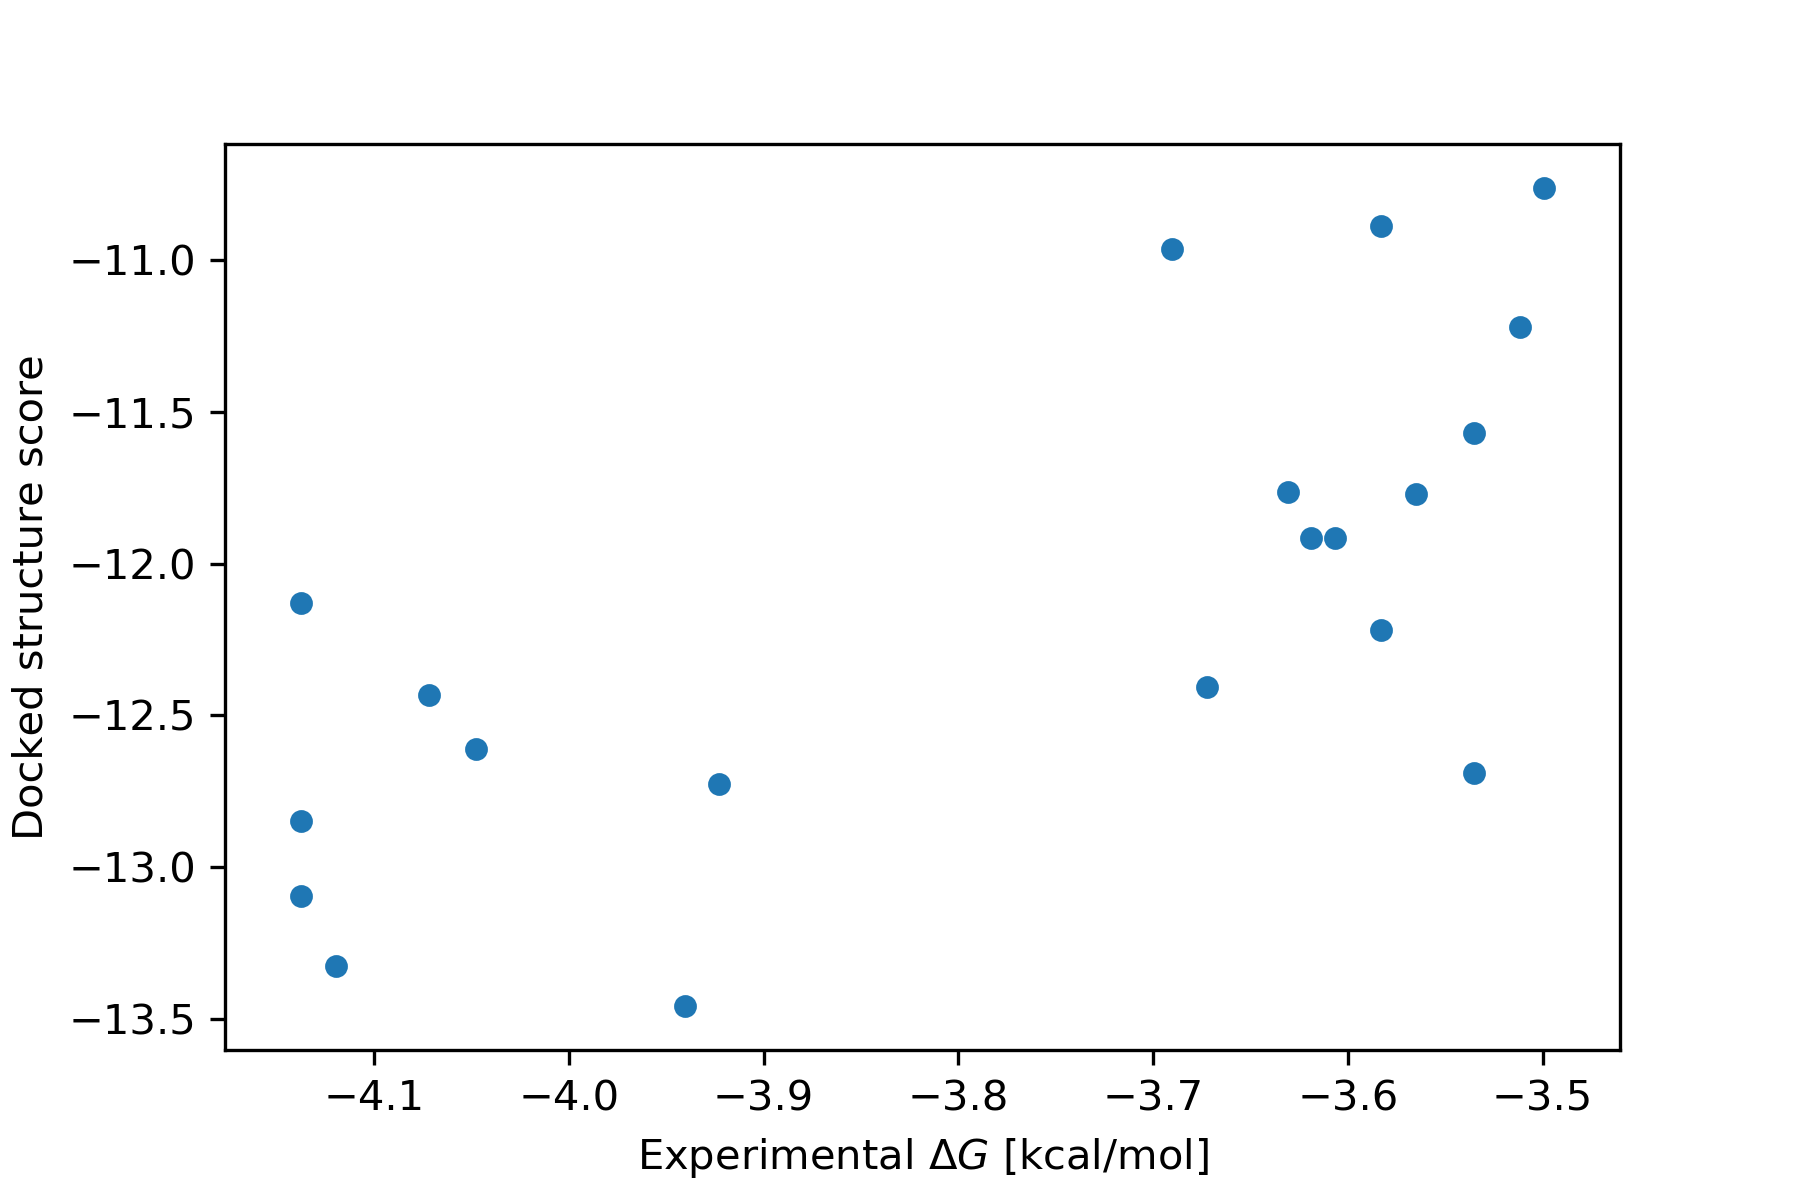
\includegraphics[width=\columnwidth]{docking}
  \caption{Plot of scores from docking the intercalators to the 1Z3F crystal structure. The ranking inside the 4 and 5 ring scaffold is poor, but there is a clear separation between the two intercalator types. This is in line with what we expect from the scoring method.}
  \label{fig:docking}
\end{figure}

\section{ESMACS}

In the past, there has been a number of MMPBSA type calculations for DNA intercalator systems. A large majority of these studies only takes into account just a few (one to three) intercalators binding to the DNA, and does not compare to experimental studies. We obtained a correlation Pearson coefficient of $r_p=0.70$ across the 10 planar molecules for the 3 trajectory calculation.

\subsubsection{Convergence}

It is important to assess the sampling efficiency and converge of the predicted free energy values in order for the results to be reliable and reproducible.
First, the comparison in convergence between a single trajectory approach and an ensemble of trajectories is compared for the MMPBSA and NMODE analysis methods in the context of free energy calculations. As the improvement in ensemble methods was evident, we investigated the length of each replica, extending the simulations from the original 5 ns simulation to 20 ns for each of the 25 replicas. It was important to sample the system long enough to cover a large part of the phase space, but not to oversample in places where the methods is no longer valid, for example during a de-intercalation pathway.

\subsubsection{Replica size and bootstrapped error}



\begin{figure}
  \begin{tikzpicture}
\begin{axis}[
  xlabel=Number of replicas,
  ylabel={Error (kcal/mol)},
  ]
  
  \addplot table {bootstrap.csv};
  
\end{axis}
\end{tikzpicture}
  \caption{Bootstrapped error as a function of replica size. }
  \label{fig:bootstrap}
\end{figure}

\subsubsection{Predicting the ranking}

The experimental free energy values are between \SIlist{-3.69;-3.50}{\kilo\calorie\per\mole}, making them hard to differentiate computationally. Approximate methods, like ESMACS, that are based on MMPBSA and NMODE for the free energy and entropy contribution, respectively do not have the resolution to differentiate experimental values at this scale. Nonetheless, correct error control and ensemble based calculations can give meaningful results relative to each other, i.e. ranking the intercalators based on their free energies will be comparable to experimental ranking.

% In methods talk about 1, 2, 3 trajectory

We have run 1, 2 and 3 trajectory calculations and as seen in Figure~\ref{fig:mmpbsa} the correlation improves, with the 3 trajectory being the most accurate with a correlation coefficient of $r_p=0.70$. The small interval of the experimental values suggests that the intercalators are very closely binding to the DNA. 

% This is a new subsection describing the energy components. P
% Check the 

The correlation achieved with ESMACS in this study suggests that one of the underlying forces (electrostatic, vdW, or internal energy) dominates the interaction gradient between the intercalators, and that signal is picked up by the MMPBSA calculation. Figure~\ref{fig:corrmat} shows the spread of the free energy values of the different components. Previous studies \cite{} have shown that vdW interactions contribute most to the binding energy of the intercalators in absolute terms. However, the correlation of the different components to the total binding energy shows that the internal energy (the sum of bond, angle, and torsion terms) correlate ~surprisingly~ with the total. 
% Induce fit, what it is?
This further supports our claim that the intercalation is an induced fit inside the two base-pairs.

% Methods
Each ESMACS calculation was run 25 times, the only difference being the random seed at the start of the simulation. 

% Beginning, quality of simulations, 
Variations in the results from the different replica was used to evaluate the error on the predicted free energy. Figure~\ref{fig:bootstrap} shows the bootstrapped error as a function of the number of replicas. There is a leveling off at around 20 replicas, with 25 replicas showing consistently low error bars.

% Energy contribution section
NMODE analysis was performed to include an approximation to the entropy contribution. Results show that including NMODE does not improve the ranking. 

% Convergence

% The original ESMACS protocol by \cite{} et al. 

\begin{figure}[h!]
	\documentclass[margin=0.1in]{article}

\usepackage{pgfplots}
\usepackage{pgfplotstable}
\pgfplotsset{compat=newest}


\usepackage{amsmath}
\usepackage{tikz}
\usetikzlibrary{positioning, calc}

\pgfmathsetmacro{\s}{0.5}
\pgfmathsetmacro{\r}{0.5cm}

\usepackage[caption=false]{subfig}

\begin{document}

\begin{figure}
  
\subfloat{%
\begin{tikzpicture}%3traj
\begin{axis}[
  scale=0.7,
  xtick distance = {0.1},
  ytick distance = {1},
  %xlabel={\phantom{nothing}}, 
  %ylabel={Calculated $\Delta$G (\si{\kilo\calorie\per\mole})},
  legend pos=south east]
  
  \addplot[blue!70!white] table [col sep=comma, x=exp, y={create col/linear regression={y=dg_3_traj}}] {4-ring-mmpbsa.csv};
  % \addplot[red!70!white] table [col sep=comma, x=exp, y={create col/linear regression={y=dg_3_traj_nmode}}] {4-ring-mmpbsa.csv};

  \addplot[blue, mark=*, only marks, error bars/.cd,
          x dir=both, x explicit,
          y dir=both, y explicit,] table 
          [col sep=comma, x=exp, y=dg_3_traj, y error=dg_3_traj_err, x error=exp_err] {4-ring-mmpbsa.csv};
  % \addplot[red, mark=*, only marks, error bars/.cd,
  %         x dir=both, x explicit,
  %         y dir=both, y explicit,] table[col sep=comma, x=exp, y=dg_3_traj_nmode, y error=dg_3_traj_err, x error=exp_err] {4-ring-mmpbsa.csv};
  
  \legend{3 trajectory, $R=0.70$}%, w/ n-mode}

\end{axis}  
\end{tikzpicture}%
}
\subfloat{%
\begin{tikzpicture}%3traj-nmode
\begin{axis}[
  scale=0.7,
  xtick distance = {0.1},
  ytick distance = {1},
  %xlabel={\phantom{nothing}}, 
  %ylabel={Calculated $\Delta$G (\si{\kilo\calorie\per\mole})},
  legend pos=south east]
  
  \addplot[red!70!white] table [col sep=comma, x=exp, y={create col/linear regression={y=dg_3_traj_nmode}}] {4-ring-mmpbsa-failednmode.csv};
  % \addplot[red!70!white] table [col sep=comma, x=exp, y={create col/linear regression={y=dg_3_traj_nmode}}] {4-ring-mmpbsa.csv};

  \addplot[red, mark=*, only marks, error bars/.cd,
          x dir=both, x explicit,
          y dir=both, y explicit,] table 
          [col sep=comma, x=exp, y=dg_3_traj_nmode, y error=dg_3_traj_err, x error=exp_err] {4-ring-mmpbsa-failednmode.csv};
  % \addplot[red, mark=*, only marks, error bars/.cd,
  %         x dir=both, x explicit,
  %         y dir=both, y explicit,] table[col sep=comma, x=exp, y=dg_3_traj_nmode, y error=dg_3_traj_err, x error=exp_err] {4-ring-mmpbsa.csv};
  
  \legend{3 trajectory + nmode, $R=0.62$}%, w/ n-mode}

\end{axis}  
\end{tikzpicture}
}

\subfloat{%
\begin{tikzpicture}%2traj
\begin{axis}[
  scale=0.7,
  xtick distance = {0.1},
  ytick distance = {1},
  %xlabel=Experimental $\Delta$G (\si{\kilo\calorie\per\mole}), 
  %ylabel={Calculated $\Delta$G (\si{\kilo\calorie\per\mole})},
  legend pos=south east
  ]
  
  \addplot[blue!70!white] table [col sep=comma, x=exp, y={create col/linear regression={y=dg_2_traj}}] {4-ring-mmpbsa.csv};    
  % \addplot[red!70!white] table [col sep=comma, x=exp, y={create col/linear regression={y=dg_2_traj_nmode}}] {4-ring-mmpbsa.csv};

  \addplot[blue, mark=*, only marks, only marks, error bars/.cd,
          x dir=both, x explicit,
          y dir=both, y explicit,] table[col sep=comma, x=exp, y=dg_2_traj, y error=dg_2_traj_err, x error=exp_err] {4-ring-mmpbsa.csv};
  % \addplot[red, mark=*, only marks, only marks, error bars/.cd,
  %         x dir=both, x explicit,
  %         y dir=both, y explicit,] table[col sep=comma, x=exp, y=dg_2_traj_nmode, y error=dg_2_traj_err, x error=exp_err] {4-ring-mmpbsa.csv};
  \legend{2 trajectory, $R=0.64$}%, w/ n-mode}

\end{axis}  
\end{tikzpicture}%
}
\subfloat{%
\begin{tikzpicture}%2traj-nmode
\begin{axis}[
  scale=0.7,
  xtick distance = {0.1},
  ytick distance = {1},
  %xlabel=Experimental $\Delta$G (\si{\kilo\calorie\per\mole}), 
  %ylabel={Calculated $\Delta$G (\si{\kilo\calorie\per\mole})},
  legend pos=south east
  ]
  
  \addplot[red!70!white] table [col sep=comma, x=exp, y={create col/linear regression={y=dg_2_traj_nmode}}] {4-ring-mmpbsa-failednmode.csv};    
  % \addplot[red!70!white] table [col sep=comma, x=exp, y={create col/linear regression={y=dg_2_traj_nmode}}] {4-ring-mmpbsa.csv};

  \addplot[red, mark=*, only marks, only marks, error bars/.cd,
          x dir=both, x explicit,
          y dir=both, y explicit,] table[col sep=comma, x=exp, y=dg_2_traj_nmode, y error=dg_2_traj_err, x error=exp_err] {4-ring-mmpbsa-failednmode.csv};
  % \addplot[red, mark=*, only marks, only marks, error bars/.cd,
  %         x dir=both, x explicit,
  %         y dir=both, y explicit,] table[col sep=comma, x=exp, y=dg_2_traj_nmode, y error=dg_2_traj_err, x error=exp_err] {4-ring-mmpbsa.csv};
  \legend{2 trajectory + nmode, $R=0.50$}%, w/ n-mode}

\end{axis}  
\end{tikzpicture}
}

\subfloat{%
\begin{tikzpicture}%1traj
\begin{axis}[
  scale=0.7,
  xtick distance = {0.1},
  ytick distance = {1},
  %xlabel={\phantom{nothing}}, 
  %ylabel={Calculated $\Delta$G (\si{\kilo\calorie\per\mole})},
  legend pos=south east
  ]
  
  \addplot[blue!70!white] table [col sep=comma, x=exp, y={create col/linear regression={y=dg_1_traj}}] {4-ring-mmpbsa.csv};    
  % \addplot[red!70!white] table [col sep=comma, x=exp, y={create col/linear regression={y=dg_2_traj_nmode}}] {4-ring-mmpbsa.csv};

  \addplot[blue, mark=*, only marks, only marks, error bars/.cd,
          x dir=both, x explicit,
          y dir=both, y explicit,] table[col sep=comma, x=exp, y=dg_1_traj, y error=dg_1_traj_err, x error=exp_err] {4-ring-mmpbsa.csv};
  % \addplot[red, mark=*, only marks, only marks, error bars/.cd,
  %         x dir=both, x explicit,
  %         y dir=both, y explicit,] table[col sep=comma, x=exp, y=dg_2_traj_nmode, y error=dg_2_traj_err, x error=exp_err] {4-ring-mmpbsa.csv};
  \legend{1 trajectory, $R=0.64$}%, w/ n-mode}
\end{axis}  
\end{tikzpicture}%
}
\subfloat{%
\begin{tikzpicture}%1traj-nmode
\begin{axis}[
  scale=0.7,
  xtick distance = {0.1},
  ytick distance = {1},
  %xlabel={\phantom{nothing}}, 
  %ylabel={Calculated $\Delta$G (\si{\kilo\calorie\per\mole})},
  legend pos=south east
  ]
  
  \addplot[red!70!white] table [col sep=comma, x=exp, y={create col/linear regression={y=dg_1_traj_nmode}}] {4-ring-mmpbsa-failednmode.csv};    
  % \addplot[red!70!white] table [col sep=comma, x=exp, y={create col/linear regression={y=dg_2_traj_nmode}}] {4-ring-mmpbsa.csv};

  \addplot[red, mark=*, only marks, only marks, error bars/.cd,
          x dir=both, x explicit,
          y dir=both, y explicit,] table[col sep=comma, x=exp, y=dg_1_traj_nmode, y error=dg_1_traj_err, x error=exp_err] {4-ring-mmpbsa-failednmode.csv};
  % \addplot[red, mark=*, only marks, only marks, error bars/.cd,
  %         x dir=both, x explicit,
  %         y dir=both, y explicit,] table[col sep=comma, x=exp, y=dg_2_traj_nmode, y error=dg_2_traj_err, x error=exp_err] {4-ring-mmpbsa.csv};
  \legend{1 trajectory + nmode, $R=0.39$}%, w/ n-mode}
\end{axis}  
\end{tikzpicture}
}
\end{figure}

\end{document}
	\caption{Correlation between one (bottom), two (middle) and three (top) trajectory calculations and experiment. Values are presented for NMODE (red) analysis and without NMODE (blue). The best Pearson correlation is for the NMODE-less values starting from \num{0.64} for the 1, and 2 trajectory and \num{0.70} for the 3 trajectory. The NMODE calculations have a Pearson correlation of \numlist{0.39; 0.5; 0.62} for the 1, 2, and 3 trajectory calculations respectively.}
	\label{fig:mmpbsa}
\end{figure}


\section{TIES}

Relative alchemical free energy calculations were done between five pairs of the intercalator from the original experimental study. As discussed above, there are two groups of intercalator there: the four and five membered ring scaffolds. Pairs were selected based on two criteria: first to maximise the experimental free energy difference and second to sample all three possible combinations of transformation (between the 4 ring systems, 5 ring systems, and a transformation from 4 ring to 5 ring). 

As seen in figure~\ref{fig:ties} the correlation to experiment is poor. This can be for a number of reasons, but investigating more systems could be insightful. The experimental results for this study indicate binding affinities that are very close to each other, and even the best methods will struggle to differentiate between them. In the future we will collect and simulate intercalator ligand systems with experimental free energy differences large enough to be probed computationally. The simulations do converge as seen in figure~\ref{fig:ties_conv} well before the end of the simulation time. Still, TIES does produce more accurate results then the more approximate methods like ESMACS or docking. The root mean squared error on this small set of transformations is 0.41 kcal/mol.

\begin{figure}
  \centering
  \begin{tikzpicture}
\begin{axis}[
  ylabel=Predicted $\Delta \Delta G$,
  xlabel=Experimental $\Delta \Delta G$,
  ]
  
  \addplot[blue, mark=*, only marks] table {ties.csv};
  
\end{axis}  
\end{tikzpicture}
  \caption{Correlation plot comparing the experiment free energy difference with the calculated values via TIES. The experimental values are too close to each other, and the difference is smaller than the resolution of the TIES method given the 5 replicas used here. Furthermore the experimental error becomes large when we take the free energy difference between two values.}
  \label{fig:ties}
\end{figure}

\begin{figure}
  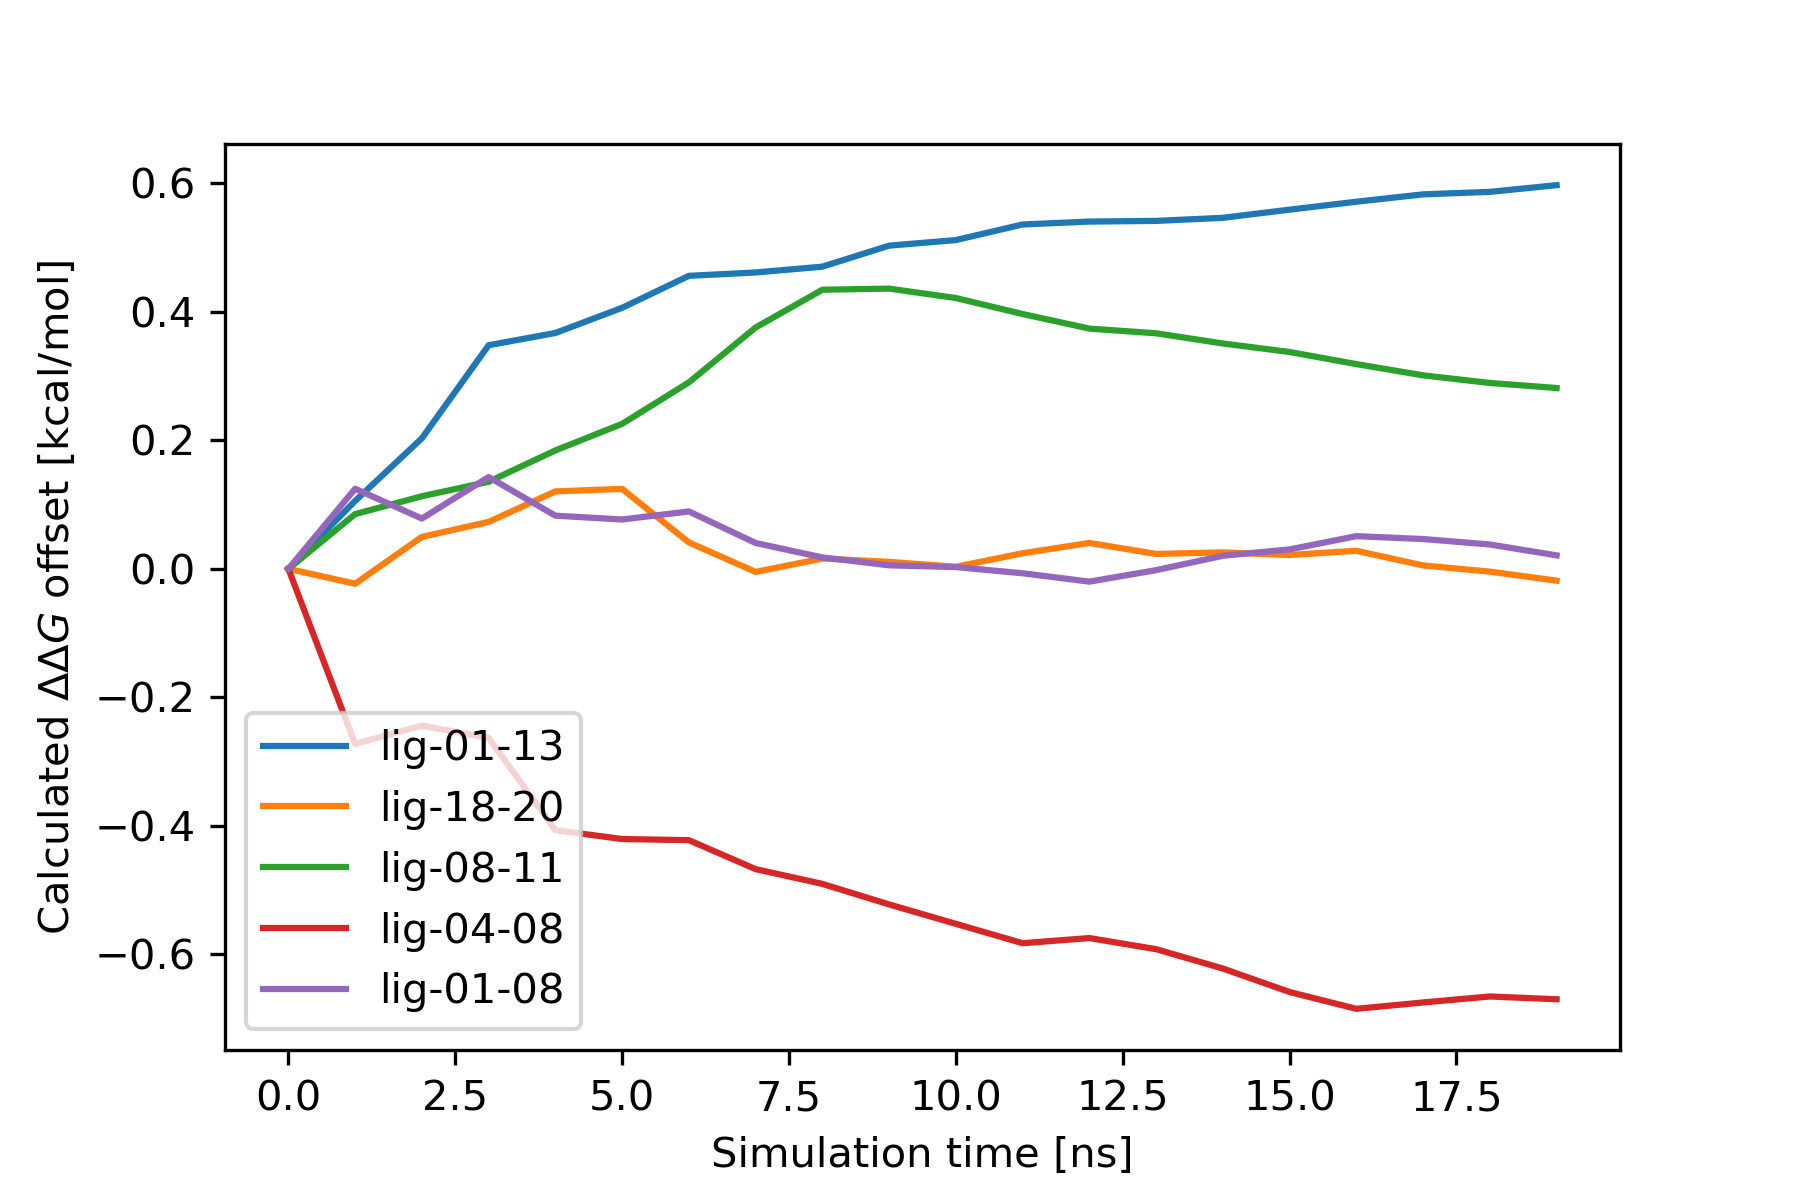
\includegraphics[width=\columnwidth]{ties_conv.png}
  \caption{Time evolution of the free energy difference for the five intercalator pairs investigated. The results are levelled off indicating that we reached converged values. The values are offset so they all start at point zero for illustrative purposes.}
  \label{fig:ties_conv}
\end{figure}



\chapter{Conclusion}


%\bibliography{mybib}
%\bibliographystyle{plain}

\end{document}